\begin{appendices}
    \chapter*{Anexo II}
    \addcontentsline{toc}{chapter}{Anexo II}
    \label{cap:anexoII}
\setcounter{page}{1}
Durante las primeras fases del desarrollo del TFG, se desarrolló un teleoperador\footnote{\url{https://github.com/RoboticsLabURJC/2022-tfg-barbara-villalba/tree/main/src/teleop_drone}} 
para analizar el comportamiento del dron frente a los comandos de posición y velocidades lineales y angulares.
Para la implementación del mismo, se utilizó el simulador Gazebo junto con PX4 Autopilot, Mavros y ROS. 

En primer lugar, se llevó a cabo la configuración del dron, específicamente el modelo Iris, dentro del archivo de configuraciones del propio launcher de PX4. Una vez cargado 
el modelo en Gazebo, se procedió a realizar la tarea de teleoperación. Para el desarrollo de la aplicación de teleoperación, se desarrollaron 
dos nodos diferentes: la interfaz, en la cual se visualiza la imagen de la cámara abordo del dron junto con sliders y botones para comandar velocidades lineales y angulares, despegue y aterrizaje, y
el teleoperador, donde se procesan los datos que se reciben a través de la interfaz. 

El nodo de la interfaz, esta construida a partir de la biblioteca PyQt5, donde se captura la imagen del dron calculando sus frames por segundo junto con la creación diferentes botones y sliders para comandar 
la orden que se quiere seguir. Entre los botones, se implementan las funciones de despegue (Take Off) y aterrizaje (Land), junto con los modos de control: posición y velocidad.
. Respecto a los sliders, se tiene en total
4: control de posición en el eje x, control de posición en el eje z, control de velocidad lineal en el eje x e control de velocidad angular en el eje z.  Con este nodo se envían las ordenes que 
posteriormente serán procesadas en el nodo de la teleoperación.

En el nodo de teleoperación, se gestionan las peticiones realizadas desde la interfaz mediante la subscripción a través de topics. Con dichos topics, se puede determinar qué comando
se desea enviar al dron. Para el control tanto de posición como de velocidad, junto con los comandos Take off y Land, se utilizan PX4 y Mavros. En la figura \ref{fig:Teleoperador}, 
se muestra el simulador Gazebo junto con el dron Iris y el nodo de la interfaz para comandar el comportamiento deseado del dron. Esta aplicación de teleoperación es una buena herramienta 
para el control del movimiento que se puede tener en un dron.

\begin{figure}[H]
    \centering
    \begin{minipage}{1.0\textwidth}
      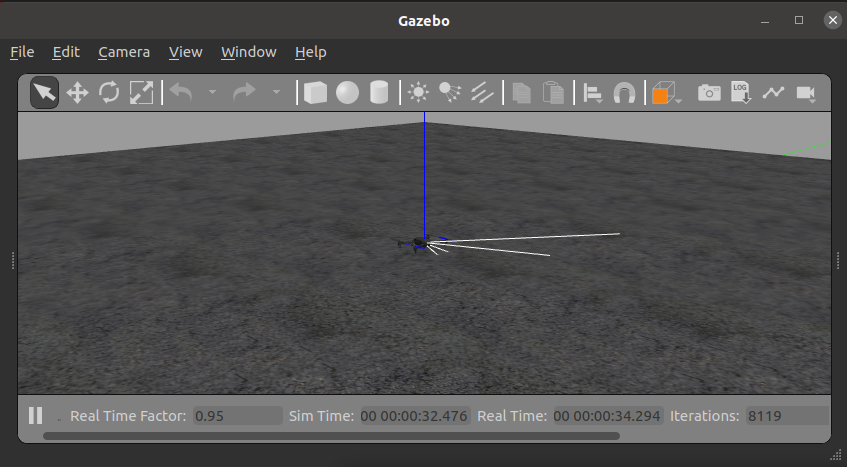
\includegraphics[width=\linewidth]{figs/anexo/gazebo.png}
    \end{minipage}
    \begin{minipage}{1.0\textwidth}
      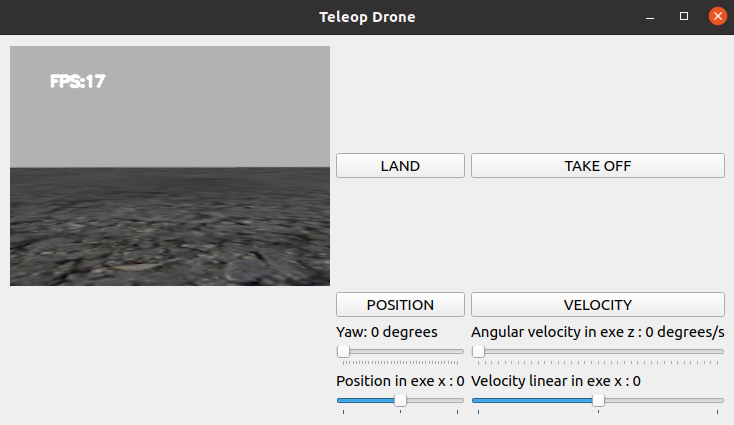
\includegraphics[width=\linewidth]{figs/anexo/interfaz.png}
    \end{minipage}
    \caption{Teleoperador}
    \label{fig:Teleoperador}
    \vspace{-1.5em}
  \end{figure}

\end{appendices}







